\documentclass[class=report,crop=false]{standalone}
\usepackage[screen]{../exo7book}

% Commande ponctuelle
\newcommand{\alenvers}[1]{\rotatebox[origin=c]{180}{#1}}
\newcommand{\vect}{\overrightarrow}

\begin{document}

%====================================================================
\chapitre{Calcul formel}
%====================================================================

%\insertvideo{s0aR-QbmTAo}{partie 5. Algèbre linéaire}

%%%%%%%%%%%%%%%%%%%%%%%%%%%%%%%%%%%%%%%%%%%%%%%%%%%%%%%%%%%%%%%%
\setcounter{section}{4}
\section{Algèbre linéaire}

L'algèbre linéaire est la partie des mathématiques consacrée à l'étude 
des matrices et des structures vectorielles.
Beaucoup de problèmes se ramènent ou s'approchent par 
des problèmes linéaires, pour lesquels il existe souvent 
des solutions efficaces.


%--------------------------------------------------------
\subsection{Opérations de base}

\begin{tp}
Soient les matrices :
$$A = 
\begin{pmatrix}
1&2&3\\
-1&0&1\\
0&1&0\\ 
\end{pmatrix}
\qquad
B = 
\begin{pmatrix}
2&-1&0\\
-1&0&1\\ 
\end{pmatrix}
\qquad
I = 
\begin{pmatrix}
1&0&0\\
0&1&0\\ 
0&0&1\\ 
\end{pmatrix}
\qquad
u = \begin{pmatrix}1\\x\\x^2\end{pmatrix}
\qquad
v = \begin{pmatrix}1\\0\\1\end{pmatrix}$$

\begin{enumerate}
  \item Calculer tous les produits possibles 
  à partir de $A,B,u$ et $v$.
  
  \item Calculer $(A-I)^7$ et en extraire le coefficient 
  de la deuxième ligne, troisième colonne.
  
  \item Calculer $A^{-1}$. Calculer la trace de $A^{-1}$
  (c'est-à-dire la somme des coefficients sur la diagonale).
\end{enumerate}
  
\end{tp}

\begin{enumerate}
  \item On définit une matrice $n$ lignes et $p$ colonnes par la commande \\
  \centerline{\codeinline{matrix(n,p,[ [ligne1],[ligne2],... ])}}
  
  En prenant les données de l'énoncé :
  \insertcode{algos/alglin-tex1.sage}{alglin.sage (1)} 
  
  On multiplie deux matrices par \codeinline{A*B}.
  Cette opération est possible seulement si le nombre de colonnes de $A$ est égal au nombre de lignes de $B$.
  Les produits possibles sont donc ici : 
  $B\times A$, $A \times u$, $A \times v$,  $B \times u$ et $B \times v$.
  
  
  \item Ayant défini la matrice identité $I$ (par \codeinline{I = identity_matrix(3)}), 
  on calcule $M = (A-I)^{7}$ par \codeinline{(A-I)^7}, ce qui renvoie
  $$(A-I)^{7} = \begin{pmatrix}-16& -46&  11\\-25& -73& 153\\32&  57& -137\\\end{pmatrix}.$$
  Le coefficient en position $(2,3)$ d'une matrice $M$ 
  est celui sur la deuxième ligne et la troisième colonne.
  Donc ici c'est $153$.
  Une matrice $A$ se comporte en \Sage\ comme une liste à double entrée et 
  on accède aux coefficients par la commande \codeinline{A[i,j]} (\codeinline{i}
  pour les lignes, \codeinline{j} pour les colonnes).
  Attention ! Les listes étant indexées à partir du rang $0$, les premières valeurs des 
  indices \codeinline{i}, \codeinline{j} sont $0$.
  Le coefficient en position $(2,3)$ s'obtient donc par la commande :\\
  \centerline{\codeinline{((A-I)^7)[1,2]}}
  Faites bien attention au décalage des deux indices.
  
  
  \item L'inverse d'une matrice \codeinline{A} se calcule par
  \codeinline{A^-1} ou \codeinline{A.inverse()}. 
  Ce qui donne 
  $$A^{-1} = \begin{pmatrix}\frac14&-\frac34&-\frac12\\0& 0& 1\\\frac14& \frac14&-\frac12\end{pmatrix}.$$
  La trace se calcule par une simple somme des éléments de la diagonale principale : \\
  \centerline{\codeinline{sum(A^(-1)[i,i] for i in range(3) )}}
  et vaut ici $-\frac14$.
  Mais on peut aussi calculer la trace avec la méthode \codeinline{trace} :\\
  \centerline{\codeinline{A.inverse().trace()}}
  qui donne encore $-\frac{1}{4}$.

\end{enumerate}

\begin{remarque*}
\sauteligne
\begin{itemize}
  \item Noter encore une fois que pour une matrice de taille $n$, les indices des lignes et colonnes 
  varient de $0$ à $n-1$.

  \item On peut préciser le corps sur lequel on travaille, 
  pour nous ce sera le plus souvent $\Kk = \Qq$. Par exemple :
  \codeinline{A = matrix(QQ, [[1,2],[3,4]])}.
  
  \item Avec \Sage\ on peut aussi définir des vecteurs par
  \codeinline{vector([x1,x2,...,xn])}.
  Un vecteur peut représenter soit un vecteur ligne, 
  soit un vecteur colonne. On peut multiplier une matrice 
  par un vecteur (à gauche ou à droite).
   
  \item Si on définit un vecteur, par exemple  
  \codeinline{v = vector([1, 2, 3, 4])} alors 
  \codeinline{L = matrix(v)} renvoie la matrice ligne correspondante.
  \codeinline{C = L.transpose()} renvoie la matrice colonne correspondante.   
\end{itemize}
\end{remarque*}

\begin{tp}
Pour une matrice $A \in M_n(\Kk)$ inversible et des vecteurs colonnes $u$ et $v$ à $n$ lignes,
%\in  \Kk^n$,
on définit $\alpha \in \Kk$ par : 
$$\alpha  = 1 + v^T A^{-1} u.$$
La formule de Sherman-Morrison affirme que si $\alpha\neq0$ alors
$$\bigg(A+u v^T\bigg)^{-1} = A^{-1} - \frac{A^{-1}u v^T A^{-1}}{\alpha}$$
Prouver par le calcul formel cette formule pour les matrices de taille 
$2\times2$ et $3\times 3$.
\end{tp}

Connaissant l'inverse de $A$, cette formule permet de calculer 
à moindre coût l'inverse d'une déformation de $A$ 
par une matrice de rang $1$.
Le code ne pose pas de problème. 

  \insertcode{algos/alglin-tex2.sage}{alglin.sage (2)}    
 
 
\begin{itemize}
  \item On commence par définir les coefficients qui seront nos 
	  %inconnues 
	  variables (ici pour $n=2$).

  
  \item On calcule $\alpha$ par la formule $\alpha = 1 + v^T A^{-1} u$,
qui est une matrice de taille $1\times1$ (\codeinline{alpha_matrice}), 
identifiée à un réel (\codeinline{alpha_reel}).
  
  \item On calcule ensuite les termes de gauche (\codeinline{B})
et droite (\codeinline{BB}) de la formule à prouver.
Pour la matrice \codeinline{C = B - BB}, on vérifie (après simplification) que tous ses coefficients sont nuls.
Ce qui prouve l'égalité cherchée.

  \item On pourrait également obtenir directement le résultat en demandant à \Sage\ : \\  
  \codeinline{C.simplify_rational() == matrix(2,2,0)}.
\end{itemize}


Pour une preuve à la main et en toute dimension, multiplier 
$\big(A+u v^T\big)$ par $A^{-1} - \frac{A^{-1}u v^T A^{-1}}{\alpha}$.

%--------------------------------------------------------
\subsection{Réduction de Gauss, calcul de l'inverse}


Le but de cette section est de mettre en \oe uvre la méthode de Gauss.
Cette méthode est valable pour des systèmes linéaires (ou des matrices) de taille quelconque, 
mais ici on se limite au calcul de l'inverse d'une matrice (qui est obligatoirement carrée). 
N'hésitez pas à d'abord relire votre cours sur la méthode de Gauss.

\begin{tp}
\sauteligne
\begin{enumerate}
  \item Réaliser trois fonctions qui transforment une matrice en fonction des 
  opérations élémentaires sur les lignes :
  \begin{itemize}
    \item $L_i \leftarrow c L_i$ avec $c \neq 0$ :
  on multiplie une ligne par un réel ;

    \item $L_i \leftarrow L_i+ c L_j$ :
  on ajoute à la ligne $L_i$ un multiple d'une autre ligne $L_j$ ;

    \item $L_i \leftrightarrow L_j$ : on échange deux lignes.
  \end{itemize}

  \item À l'aide de ces transformations élémentaires, transformer par la méthode de Gauss
  une matrice inversible en une matrice échelonnée (c'est-à-dire ici, en partant d'une matrice carrée,
  obtenir une matrice triangulaire supérieure).
  
  \item Toujours à l'aide de ces transformations et de la méthode de Gauss, transformer 
  cette matrice échelonnée en une matrice échelonnée et réduite
  (c'est-à-dire ici, en partant d'une matrice inversible, obtenir l'identité).
  
  \item La méthode de Gauss permet de calculer l'inverse d'une matrice $A$ :
  \begin{itemize}
    \item Partant de $A$, on pose $B = I$ la matrice identité.
    \item Par la méthode de Gauss et des opérations élémentaires,
 on transforme $A$ en 
    la matrice $I$. 
    \item On applique exactement les mêmes transformations à la matrice $B$.
    \item Lorsque $A$ s'est transformée en $I$ alors $B$ s'est transformée en $A^{-1}$.
  \end{itemize}
  Modifier légèrement vos deux fonctions (issues des questions 2. et 3.) afin 
  de calculer l'inverse d'une matrice.
\end{enumerate}
\end{tp}

Voici une matrice $A$, sa forme échelonnée, sa forme échelonnée réduite (l'identité), et son inverse:
$$
A = \begin{pmatrix}
1  &  2  &  3\\
-1  &  0  &  1\\
0  &  1  &  0\\
\end{pmatrix}\qquad
\begin{pmatrix}
1  &  2  &  3\\
0  &  2  &  4\\
0  &  0 & -2\\
\end{pmatrix}\qquad
\begin{pmatrix}
1 & 0 & 0\\
0 & 1 & 0\\
0 & 0 & 1\\
\end{pmatrix}\qquad
A^{-1} = \begin{pmatrix}
\frac14 & -\frac34 & -\frac12\\
0  &  0  &  1\\
\frac14  & \frac14 & -\frac12\\ 
\end{pmatrix}$$


\begin{enumerate}
  \item Voici la fonction pour la deuxième opération : $L_i \leftarrow L_i+ c L_j$.
  
  \insertcode{algos/gauss-tex1.sage}{gauss.sage (1)}    
   
  \codeinline{A[i,:]} correspond à la ligne \codeinline{i} (les deux points signifiant 
  de prendre tous les indices des colonnes).
  Lorsque l'on exécute cette fonction sur une matrice $A$ cela modifie la matrice (voir la 
  remarque plus bas). En particulier cette fonction ne renvoie aucune valeur.

  Les autres opérations \codeinline{op1(A, i, c)}, \codeinline{op3(A, i, j)}
  se définissent de manière analogue.
  
  
  \item 
  Il s'agit de traduire la première partie de la méthode de Gauss.
  Pour chaque colonne $p$ en partant de la plus à gauche :
  \begin{enumerate}
    \item on cherche un coefficient non nul dans cette colonne ;
    \item on place ce coefficient en position de pivot $(p,p)$, 
    en permutant deux lignes par la troisième opération élémentaire ;
    \item on annule, un par un, les coefficients qui sont sous ce pivot, par des opérations élémentaires :
    $L_i \leftarrow L_i+ c L_p$ où $c = -\frac{a_{i,p}}{a_{p,p}}$. 
  \end{enumerate}
  
  \insertcode{algos/gauss-tex2.sage}{gauss.sage (2)}

  \item Pour passer à une forme réduite, on parcourt les colonnes en partant de la droite : 
  \begin{enumerate}
    \item on commence par multiplier la ligne du pivot pour avoir un pivot valant $1$ ;
    \item on annule, un par un, les coefficients qui sont au-dessus de ce pivot.
  \end{enumerate}
  
  \insertcode{algos/gauss-tex3.sage}{gauss.sage (3)}
  
  
  \item Pour calculer l'inverse, on définit deux nouvelles fonctions \codeinline{echelonne_bis(A,B)} et
   \codeinline{reduite_bis(A,B)}
  qui modifient chacune les deux matrices $A$ et $B$.
  À chaque fois que l'on effectue une opération sur $A$, on effectue la même opération sur $B$.
  Par exemple, la dernière boucle de \codeinline{echelonne_bis}
  contiendra les lignes \codeinline{op2(A, i, p, c)} et \codeinline{op2(B, i, p, c)}.
  C'est bien le même coefficient $c = -\frac{a_{i,p}}{a_{p,p}}$ pour les deux opérations. 
  On obtient alors l'inverse comme ceci :
  \insertcode{algos/gauss-tex4.sage}{gauss.sage (4)}
  
\end{enumerate}

\begin{remarque*}
Si on pose 
\codeinline{A = matrix( [[1,2],[3,4]] )}, puis \codeinline{B = A},
puis que l'on modifie la matrice $A$ par \codeinline{A[0,0]= 7}. 
Alors la matrice \codeinline{B} est aussi modifée !

Que se passe-t-il ?
\begin{itemize}
  \item \codeinline{A} ne contient pas les coefficients de la matrice, mais 
  l'adresse où sont stockés ces coefficients (c'est plus léger de manipuler 
  l'adresse d'une matrice que toute la matrice).
  
  Comme \codeinline{A} et \codeinline{B} pointent 
  vers la même zone qui a été modifiée, 
  les deux matrices \codeinline{A} et \codeinline{B} sont modifiées.
  
  \item Pour pouvoir définir une copie de \codeinline{A}, avec une nouvelle 
  adresse mais les mêmes coefficients, on écrit \codeinline{AA = copy(A)}.
  Les modifications sur \codeinline{AA} ne changeront pas \codeinline{A}.
\end{itemize}
\end{remarque*}

%--------------------------------------------------------
\subsection{Application linéaire, image, noyau}



\begin{tp}
Soit $f : \Rr^3 \to \Rr^4$ l'application linéaire définie par
$$f : \begin{pmatrix}x\\y\\z\end{pmatrix}
\longmapsto 
\begin{pmatrix}
x+2z\\
5x+2y+2z\\
2x+y\\
x+y-2z
\end{pmatrix}.$$
\begin{enumerate}
  \item Expliciter la matrice $A$ de $f$ (dans les bases canoniques).
  Comment s'écrit alors l'application $f$ ?
    
  \item Calculer une base du noyau de $f$. L'application linéaire
  $f$ est-elle injective ?
  
  \item Calculer une base de l'image de $f$. L'application linéaire
  $f$ est-elle surjective ?
\end{enumerate}
\end{tp}


%
%Il faut d'abord comprendre une subtilité.
%\begin{itemize}
%  \item En mathématiques, l'application linéaire associée à une matrice $A \in M_{n,p}$
%est définie par $X \mapsto Y = AX$ où $X$ est un vecteur colonne à $p$ composantes
%et $Y$ un vecteur colonne à $n$ composantes.
%  
%  \item \Sage\ préfère travailler avec les vecteurs lignes. Ainsi étant donnée une matrice
%$B$, \Sage\ considère que l'application est $X' \mapsto Y' = X' B$ où $X'$ et $Y'$ 
%sont cette fois des vecteurs lignes.
%
% \item Pour passer d'une convention à l'autre, il suffit de demander à \Sage\ de faire les calculs pour $A^T$.
%En effet \Sage\ considère alors que l'application linéaire associée à $A^T$ est
%$X' \mapsto X' A^T$. Comme $X'$ est un vecteur ligne, on note $X = X'^{T}$ 
%le même vecteur considéré comme un vecteur colonne.
%L'application devient alors $X^T \mapsto X^TA^T = (AX)^T$, ce qui en termes de vecteurs colonnes s'écrit
%$X \mapsto AX$ ; on retrouve ainsi notre application linéaire initiale.
%\end{itemize}


%Une fois que l'on a bien compris cette subtilité, il suffit de 
%laisser la machine faire les calculs.

\begin{enumerate}
  \item La matrice associée est
  $$A = \begin{pmatrix}1&0&2\\5&2&2\\2&1&0\\1&1&-2\\\end{pmatrix}.$$
  L'application linéaire $f$ est alors définie par $X \mapsto Y = AX$.
  Voici l'implémentation avec un exemple de calcul. 
  \insertcode{algos/matlin-tex1.sage}{matlin.sage (1)}    
 
  \item et 3.
  %On pose $A' = A^T$ alors le noyau et l'image qui nous intéressent, sont ceux calculés par \Sage\ pour $A'$.
  Le noyau s'obtient par la commande \codeinline{right_kernel()} et l'image par la commande
  \codeinline{column_space()} car l'image est
  exactement le sous-espace vectoriel engendré par les vecteurs colonnes de la matrice.
  
  \insertcode{algos/matlin-tex2.sage}{matlin.sage (2)}    
  \begin{itemize}
    \item Le noyau est un espace vectoriel de dimension $1$ dans $\Rr^3$ engendré par 
  $\begin{pmatrix}2\\-4\\-1\end{pmatrix}$. 
  Le noyau n'étant pas trivial, l'application $f$ n'est pas injective.
  
    \item   L'image est un espace vectoriel de dimension $2$ dans $\Rr^4$, dont une base   
  est :
  $$\left( 
  \begin{pmatrix}2\\0\\-1\\ -3\end{pmatrix},
  \begin{pmatrix}0\\2\\ 1\\ 1\end{pmatrix}\right).$$
  L'image n'étant pas $\Rr^4$ tout entier, l'application $f$ n'est pas non plus surjective.
  
    \item On peut tester si un vecteur donné est dans un sous-espace. Si on pose par exemple 
      \codeinline{X = vector(K,[1,5,2,1])} alors le test \og \codeinline{X in Im} \fg{}
      renvoie vrai. Ce vecteur est donc bien un élément de l'image de $f$. 
  \end{itemize}
 
\end{enumerate}



Attention ! Il ne faut pas utiliser directement les méthodes \codeinline{kernel()}
et \codeinline{image()} car \Sage\ préfère travailler avec les vecteurs lignes et donc ces méthodes calculent le \emph{noyau à gauche} (c'est-à-dire l'ensemble des $X$ tels que $XA=0$)
et l'\emph{image à gauche} (c'est-à-dire l'ensemble des $Y=XA$). Si vous souhaitez utiliser ces méthodes pour calculer le noyau et l'image avec notre convention habituelle (c'est-à-dire à droite) il faut le faire sur la transposée de $A$ :
 \insertcode{algos/matlin-tex3.sage}{matlin.sage (3)}   

%--------------------------------------------------------
\subsection{Méthodes des moindres carrés}

Si on veut résoudre un système linéaire avec plus d'équations que d'inconnues 
alors il n'y a pas de solution en général. On aimerait pourtant parfois trouver 
ce qui s'approche le plus d'une solution.
Formalisons ceci : 
soit $A \in M_{n,p}(\mathbb R)$ avec $n \ge p$ une matrice à coefficients réels, 
$X$ un vecteur inconnu de taille $p$ et
$B$ un vecteur de taille $n$.
Il n'y a en général pas de solution $X$
au système $AX=B$, mais on aimerait que 
$AX-B$ soit le plus proche du vecteur nul.
Ainsi, une \defi{solution des moindres carrés} est un vecteur $X$ 
tel que $\| AX -B \|$ soit minimale, où la norme considérée est la norme euclidienne.
Cette solution des moindres carrées est donnée par la formule :
\begin{equation}
\label{eq:moindrescarres}
\tag{\dag}
X = (A^TA)^{-1} A^T B
\end{equation}
(si $n \ge p$ et $A$ est de rang maximal $p$, ce qu'on suppose, alors on peut montrer que la matrice $A^TA$ est inversible).


\begin{tp}
\sauteligne
\begin{enumerate}
  \item \textbf{Régression linéaire.} 
  On considère les points $\big\{(-6,0), (-2,1), (1,2), (4,4), (6,4)\big\}$.
  Trouver la droite qui approche au mieux ces points (au sens des moindres carrés).
  
  \emph{Indications.} On pose $f(x) = a +bx$. On aimerait trouver $a,b \in \Rr$ tels que 
  $f(x_i)=y_i$ pour tous les points $(x_i,y_i)$ donnés. 
  Transformer le problème en un problème des moindres carrés : quel est le vecteur inconnu $X$ ?
  quelle est la matrice $A$ ? quel est le second membre $B$ ?
    
  \item \textbf{Interpolation polynomiale.} 
  Pour ces mêmes points, quel polynôme de degré $3$ approche 
  au mieux ces points (au sens des moindres carrés) ?
  
  \emph{Indication.} Cette fois $f(x) = a + bx + cx^2 + dx^3$.
  
  
%  \item 
\end{enumerate}
 
\end{tp}


Voici la droite demandée (à gauche) ainsi que le polynôme de degré $3$ (à droite).
\begin{center}
    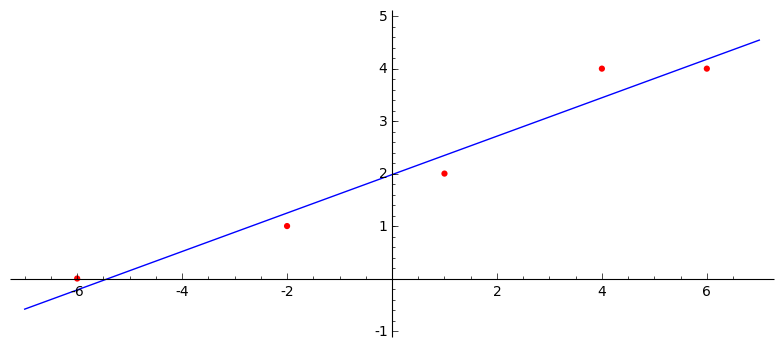
\includegraphics[scale=0.35]{figures/moindres_carres1}\quad
    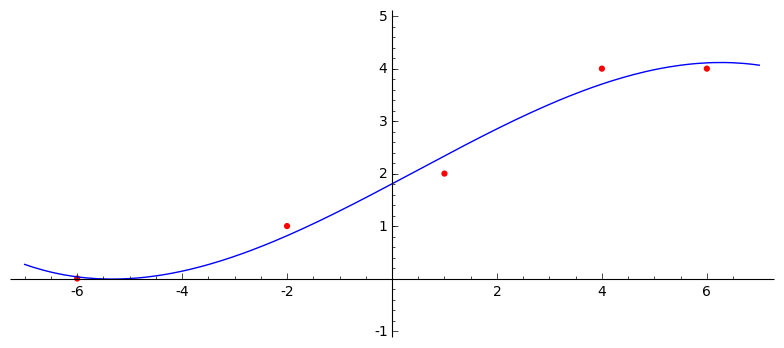
\includegraphics[scale=0.35]{figures/moindres_carres2}
\end{center} 
  
\begin{enumerate}
  \item Bien sûr les points ne sont pas alignés, donc il n'existe 
  pas de droite passant par tous ces points.
  On cherche une droite d'équation $y = a +bx$ qui minimise (le carré de) la distance
  entre les points et la droite. Posons $f(x) = a + bx$.
  
  Alors pour nos $n$ points $(x_i,y_i)$ donnés, on voudrait $f(x_i)=y_i$. 
  $$
  \left\{ 
  \begin{array}{ccl}
  f(x_1) &=& y_1 \\
  f(x_2) &=& y_2 \\
  \vdots && \vdots\\
  f(x_n) &=& y_n \\
  \end{array}
  \right.
  \quad
  \iff
  \quad
  \left\{ 
  \begin{array}{ccl}
  a +b x_1 &=& y_1 \\
  a +b x_2 &=& y_2 \\
  \vdots && \vdots\\
  a +b x_n &=& y_n \\
  \end{array}
  \right.
  \quad
  \iff
  \quad 
  \begin{pmatrix}
  1 & x_1 \\
  1 & x_2 \\
  \vdots & \vdots \\
  1 & x_n \\  
  \end{pmatrix}
  \begin{pmatrix}
  a \\ b  
  \end{pmatrix}
  = 
  \begin{pmatrix}
  y_1\\
  y_2 \\
  \vdots \\
  y_n
  \end{pmatrix}
  \quad
  \iff
  \quad 
  AX = B.
  $$
  
  On résout (de façon non exacte) notre problème $AX = B$, par la formule des moindres carrés
  $X = (A^TA)^{-1} A^T B$. Comme $X = \left(\begin{smallmatrix}a\\b\end{smallmatrix}\right)$,
  on obtient l'équation $y=a+bx$ de la droite des moindres carrés (voir la figure ci-dessus).
  
   La fonction \codeinline{moindres_carres} résout le problème général des moindres carrés.
  Il reste ensuite à définir la matrice $A$ et le vecteur $B$ en fonction de notre liste de points
  afin de trouver $X$.
  Le code est le suivant :
  \insertcode{algos/moindres_carres-tex1.sage}{moindres\_carres.sage (1)} 
  

  
  \item L'idée est la même, mais cette fois les inconnues 
  sont les coefficients de la fonction
  $f(x) = a + bx +c x^2 + dx^3$ :
   $$
  \left\{ 
  \begin{array}{ccl}
  f(x_1) &=& y_1 \\
  f(x_2) &=& y_2 \\
  \vdots && \vdots\\
  f(x_n) &=& y_n \\
  \end{array}
  \right.
  \quad
  \iff
  \quad
  \left\{ 
  \begin{array}{ccl}
  a +b x_1 + c x_1^2 + d x_1^3 &=& y_1 \\
  a +b x_2 + c x_2^2 + d x_2^3 &=& y_2 \\
  \vdots && \vdots\\
  a +b x_n + c x_n^2 + d x_n^3 &=& y_n \\
  \end{array}
  \right.
  $$
  $$
  \iff
  \quad 
  \begin{pmatrix}
  1 & x_1 & x_1^2 & x_1^3\\
  1 & x_2 & x_2^2 & x_2^3 \\
  \vdots & \vdots & \vdots & \vdots\\
  1 & x_n & x_n^2 & x_n^3  \\  
  \end{pmatrix}
  \begin{pmatrix}
  a \\ b \\ c \\ d
  \end{pmatrix}
  = 
  \begin{pmatrix}
  y_1\\
  y_2 \\
  \vdots \\
  y_n
  \end{pmatrix}
  \quad
  \iff
  \quad 
  AX = B
  $$ 
  
  Voici le code pour les mêmes points et une interpolation 
  polynomiale de degré $d$ :
  \insertcode{algos/moindres_carres-tex2.sage}{moindres\_carres.sage (2)} 
    
  
\end{enumerate}

Pour conclure, voici la preuve de la formule 
(\ref{eq:moindrescarres}) des moindres carrés.
Caractérisons géométriquement la condition << $\| AX -B \|$ minimale >>.
On note $\Im A$ l'image de $A$, c'est-à-dire le sous-espace 
vectoriel engendré par les vecteurs colonnes de la matrice $A$.
Notons $p : \Rr^n \to \Rr^n$ la projection orthogonale sur $\Im A$.
Enfin, notons $Y=p(B)$ le projeté orthogonal de $B$ sur l'image de $A$. 

\myfigure{1.2}{  
  \tikzinput{fig_formel_alglin_01}
}

Comme $Y$ est dans l'image de $A$ alors il existe $X$ tel que
$AX=Y$ et $X$ est notre << solution >> cherchée.
En effet, c'est l'une des caractérisations du projeté orthogonal : 
$Y = p(B)$ est le point de $\Im A$ qui minimise la distance entre $B$ et un 
point de $\Im A$. 
  
  
  Que $Y$ soit le projeté orthogonal de $B$ sur $\Im A$ signifie
  que le vecteur $B-Y$ est orthogonal à tout vecteur de $\Im A$:
  \begin{eqnarray*}
    && \langle AV \mid B-Y \rangle = 0 \quad \forall V \in \Rr^p \\
    & \iff & \langle AV \mid B-AX \rangle = 0 \quad \forall V \in \Rr^p \quad \text{ pour } Y=AX\\
    & \iff & (AV)^T \cdot (B-AX)= 0 \quad \forall V \in \Rr^p \quad \text{ car } \langle u \mid v\rangle = u^T\cdot v\\
    & \iff & V^T  A^T (B-AX)= 0 \quad \forall V \in \Rr^p \\    
    & \iff & A^T (B-AX)= 0 \\
    & \iff & A^TAX= A^T B \\
    & \iff & X = (A^TA)^{-1} A^TB. \\    
  \end{eqnarray*} 



  
\begin{remarque*}
  Dans la dernière ligne de cette preuve, nous supposons (et admettons) que la matrice $A^TA$ est 
  inversible, ce qui est toujours vrai lorsque la matrice $A$ est de rang maximal (donc de rang $p$, 
  car ici $p \le n$).

\end{remarque*}

\finchapitre

\end{document}

